\section{On-issue tracking}

For on-issue tracking, we first divide news articles quarterly.
Then we classify news articles in each quarter group into 20 issue categories.
For each classified group, each article’s 5W1H(when, where, who, what, why, how) is extracted and counted.
The most frequent 5W1H will represent an on-issue event for the quarter.

Figure \ref{fig:onissuedia} shows the structure of the on-issue tracking process.

\begin{figure}[!htbp]
  \centering
  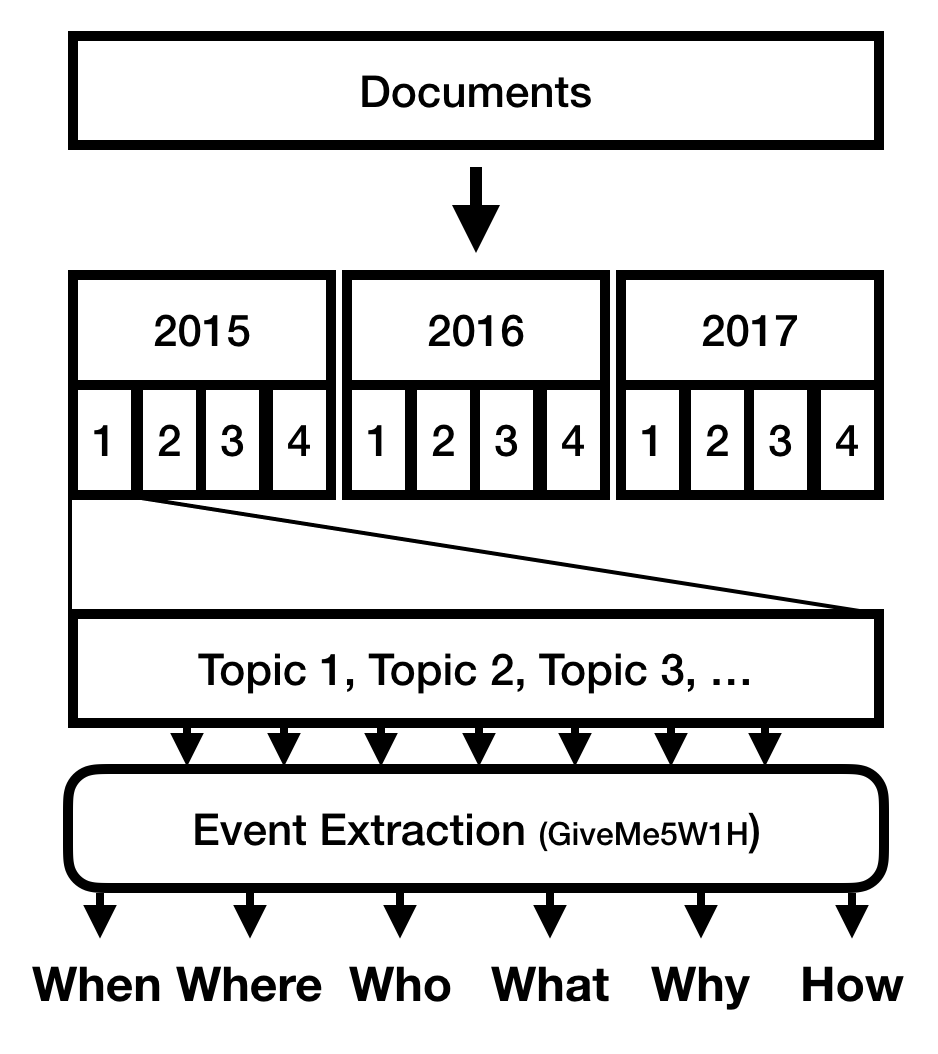
\includegraphics[width=0.8\linewidth]{on_issue_1.png}
  \caption{A brief diagram of on-issue tracking process.}
  \label{fig:onissuedia}
\end{figure}

\subsection{Quarterly Division}

We divided all news articles quarterly.
The groups contain news articles those are written in \textit{2015 Q1, 2015 Q2, …, 2017 Q4, 2018 Q1}.
\textit{2018 Q1} group contains only articles written in January, 2018,
so we merge the last group with the group \textit{2017 Q4}.
The reason why we divided the data quarterly is, the quarter is a semi-standard in the field of yearly statistics.
If we divide yearly, there will be only three groups
and it will not have high accuracy if we make a timeline of the events.
So we chose a quarterly division to make reasonable results.

\subsection{Articles in the Quarters Categorization}

With LDA model we have trained at trend analysis project,
we classify the documents in the quarter groups.
If we give a tokenized sentence to the LDA model,
the model outputs the probability for each group.
We choose the group with maximum value, and assign the document to the group.
So, for each quarter, there are 21 classified groups of news articles.

\subsection{Event Extraction}

For each group we divided from above,
we extract the events with the approach of word frequency.
For this step, we use a Python library called ``giveme5W1H''.
The library is the state-of-the-art tool for extracting
\textit{when/where/who/what/why/how} features from the document.
The library uses Stanford's CoreNLP library as its basic structure,
and give analysis results when we give a
title, lead, text, and a published date.
We decided to use columns \textit{title}, \textit{description}, \textit{body}, and a \textit{time}
from the given dataset as an input to get a result.
For each group, we count the frequencies of each feature of the articles,
and select the most frequent terms for each feature, treat them as an event.

In details, to reduce the time of event extraction,
we choose two yearly issues from the list, and do event extraction for each issue.
So each yearly issue has four event extraction result: in Q1, Q2, Q3, and Q4.
For each quarter result, we identify an event based on the result and align them on the timeline.

Table ? is an on-issue tracking of the issue MERS.
The events timeline of the issue MERS in 2015 is: 
\textbf{
Korean aid worker sent(Q1) ->
Korean government's MERS announcing ->
Korean government reports no additional MERS cases ->
Government created free medical school
}.

